\documentclass[journal,onecolumn]{IEEEtran}

\usepackage{graphicx} % Required for inserting images
\usepackage{geometry}
\usepackage{minted}
\usepackage{hyperref}
\usepackage{mathtools}
\usepackage{enumitem}
\usepackage{amssymb}
\usepackage{float}
\usepackage{caption}
\usepackage{subcaption}

\DeclareMathOperator{\dom}{\mathbf{dom}}
\DeclareMathOperator{\best}{best}
\DeclareMathOperator{\tr}{\mathbf{tr}}
\DeclareMathOperator{\argmin}{argmin}
\DeclareMathOperator{\sign}{sign}
\let\oldforall\forall
\renewcommand{\forall}{ \, \oldforall \, }

\def\BibTeX{{\rm B\kern-.05em{\sc i\kern-.025em b}\kern-.08em
    T\kern-.1667em\lower.7ex\hbox{E}\kern-.125emX}}


\begin{document}
\title{
Subgradient Methods Applied to LASSO Regression on Life Expectancy Data
}

\author{\IEEEauthorblockN{Kasey Tian}\\
\IEEEauthorblockA{\textit{Electrical and Computer Engineering} \\
\textit{Rutgers University}\\
New Brunswick, NJ, USA \\
kasey.tian@rutgers.edu}
}


\maketitle

\begin{abstract}
Subgradient methods are a powerful class of methods to optimize non-differentiable objective functions. One common application is in LASSO regression, which is a regression scheme originally designed for use with linear classifiers. We have applied subgradient methods to LASSO regression to create a linear classifier of life expectancy data to prove the efficacy of this technique.
\end{abstract}

\begin{IEEEkeywords}
optimization, subgradients, LASSO, regression
\end{IEEEkeywords}

\section{Introduction}\label{sec:intro}
Subgradient methods are a way to perform an optimization on an objective function which is not fully differentiable. For non-differentiable objective functions, traditional methods, such as gradient descent and Newton's method, are impossible to execute. They can also be combined with a wide variety of other optimization methods, and have far reaching applications. They were originally developed by Shor and others in the Soviet Union in the 1960s and 70s \cite{boydparksubgradients} \cite{boydxiaosubgradients}.

One common application of subgradient methods is in LASSO (\textbf{L}east \textbf{A}bsolute \textbf{S}hrinkage and \textbf{S}election \textbf{O}perator) regression. It is a regression analysis method which was first introduced in 1986 \cite{lassooriginal} in the field of geophysics, but was then independently rediscovered, named, and popularized in 1996 \cite{lassopaper}. It is characterized by regularization using the \(L_1\) norm, which involves the absolute value function and is therefore not fully differentiable. This makes it a prime candidate for applying subgradient methods. 

We will explore the mathematics of subgradients, subgradient methods, and LASSO in Section \ref{sec:math}. To demonstrate real implementations of subgradient methods, two examples are included. The first is a simple linear example in Section \ref{sec:linear example}. The second is using LASSO regression with a linear classifier to predict life expectancy from World Health Organization (WHO) data \cite{dataset} in Section \ref{sec:lasso}. We will analyze the results of the LASSO regression in Section \ref{sec:results}, and then conclude with some brief remarks. The source code for these implementations as well as this paper is available in Appendix \ref{sec:github}.


\section{Mathematics}\label{sec:math}
In this section we will explore the mathematics of subgradients, subgradient methods and LASSO regression.
\subsection{Subgradients}\label{sec:math subgrad}
This section is mostly adapted from \cite{boydvandenberghesubgradient}, with some supplementary material from \cite{boydparksubgradients}.
\subsubsection{Definitions}
A subgradient is defined for some convex function \(f: \mathbb{R}^n \rightarrow \mathbb{R}\) at a point \(x \in \dom f\) as a vector \(g \in \mathbb{R}^n\) such that \(\forall y \in \dom f\)
\begin{equation}\label{eq:subgradient def}
f(y) \geq f(x) + g^T (y-x) 
\end{equation}
Alternately expressed as
\begin{equation}\label{eq:modified subradient def 2}
    f(y) - f(x) \geq g^T(y-x)
\end{equation}
\begin{equation}\label{eq:modified subgradient def}
    f(x) - f(y) + g^T(y-x) \leq 0
\end{equation}
There can be multiple subgradients at a point \(x\), so we will also define the subdifferential \(\partial f(x)\) to be the set of all subgradients at \(x\).
\begin{equation}\label{eq:math subdifferential}
\partial f(x) = \bigcap_{y \in \dom f} \left\{ g : f(y) \geq f(x) + g^T (y-x)\right\}
\end{equation}
If there exists at least one subgradient at a point \(x\), we would say \(f\) is subdifferentiable at \(x\). If all points in the domain are subdifferentiable, we say that \(f\) is subdifferentiable.

\subsubsection{Example: Absolute Value}
If we consider \(g\) in \eqref{eq:subgradient def} to be a slope, we can visualize a subgradient as being some hyperplane intersecting our function at \(x\) for which all values of the function are on or above the plane. 

Let us employ this intuition to find a subgradient of the function \(f(x) = |x|\) at the point \(x=0\). Graphically, we can see in Fig. \ref{fig:abs subgradients} that many different lines satisfy this criteron.
\begin{figure}[htbp]
    \centering
    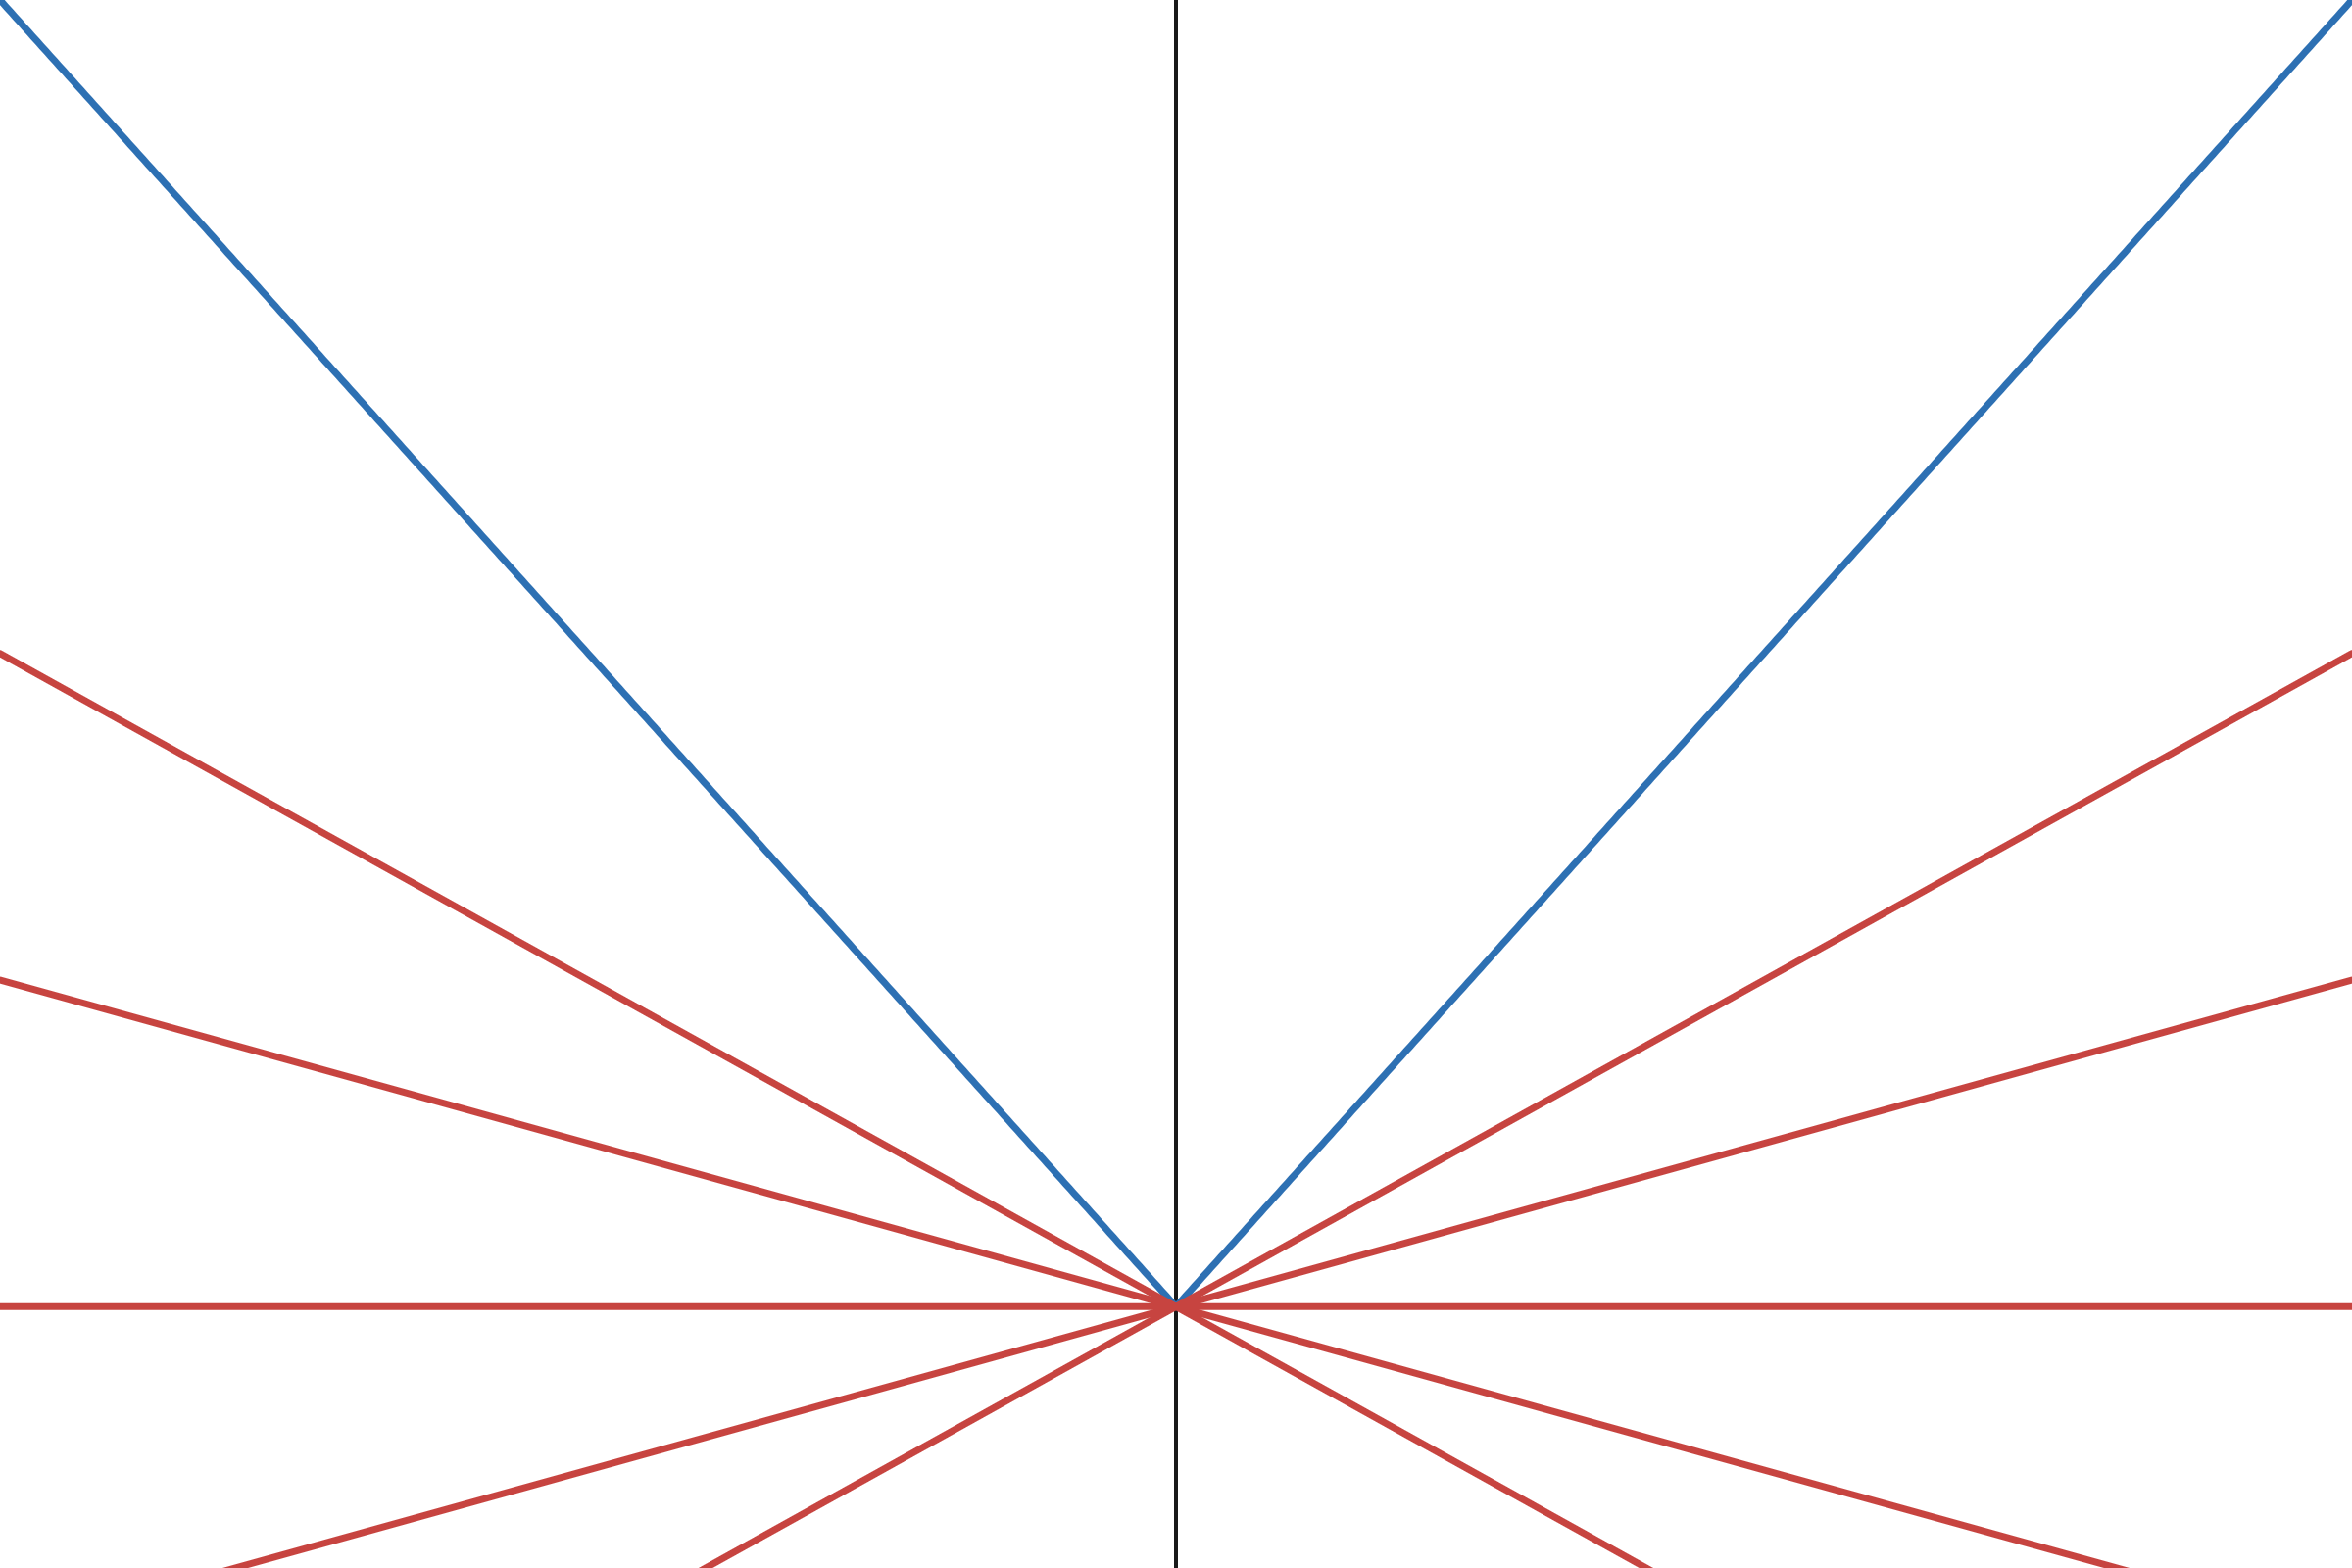
\includegraphics[width=0.5\linewidth]{Figures/abs_subgradients.png}
    \caption{Absolute value function (blue) with subgradients (red)}
    \label{fig:abs subgradients}
\end{figure}
In fact, we can say that any \(g \in [-1,1]\) would be a subgradient, and therefore \(\partial f(0) = [-1,1]\). But what about other points? For a point \(x > 0\), we can surmise that the only possible \(g = 1\), as any other value will leave some parts of our function beneath the resulting plane. Likewise for \(x < 0\), \(g = -1\). Using \eqref{eq:math subdifferential}, we can say
\begin{equation}\label{eq:abs subdifferential}
\partial f(x) = \begin{cases}
    \{-1\} & x < 0 \\
    [-1, 1] & x = 0\\
    \{1\} & x > 0
\end{cases}
\end{equation}
This can be compared against the derivative of \(f(x)\).
\begin{equation}\label{eq:abs derivative}
f'(x) = \begin{cases}
            -1 & x < 0\\
            1 & x > 0
\end{cases}
\end{equation}
We find that where the function is differentiable, the subdifferential contains only the gradient. There is only a difference where the function is not differentiable. Here we find that our set ranges between the two derivatives on either side of it. More formally, we can say that \(\partial f(x) = [a, b]\) such that
\begin{equation}\label{eq:subdifferential a def}
a = \lim_{y \rightarrow x^-} \frac{f(y)-f(x)}{y-x}
\end{equation}
\begin{equation}\label{eq:subdifferential b def}
b = \lim_{y \rightarrow x^+} \frac{f(y)-f(x)}{y-x}
\end{equation}
for one dimensional functions. We can note that for differentiable points \(a = b\), so this definition satisfies our observations.

\subsubsection{Properties}
There are a few important properties that we shall take note of. Proofs of these properties can be found in Appendix \ref{sec:subgradient properties proofs}.
\begin{itemize}
    \item If and only if the function is differentiable at \(x\), \(\partial f(x) = \{\nabla f(x)\}\)
    \item If and only if \(x^*\) is a global minimum, \(0 \in \partial f(x^*)\)
    \item \(\partial f(x)\) will always be a convex set
\end{itemize}

\subsection{Subgradient Methods}\label{sec:subgradient methods}
This section is predominantly adapted from \cite{boydparksubgradients} and \cite{boydxiaosubgradients}.

\subsubsection{Iteration Step}
Subgradient methods are a family of optimization techniques involving the same basic iteration step
\begin{equation}\label{eq:subgradient method iteration}
x^{(k+1)} = x^{(k)} - \alpha_k g^{(k)}
\end{equation}
where \(g^{(k)}\) is any subgradient at the point \(x^{(k)}\) and \(\alpha_k > 0\). There are a number of different methods of choosing \(\alpha_k\), which will be further explored in Section \ref{sec:choosing step size}. This formula can be seen to be very similar to gradient descent. In fact, can be observed that since the only subgradient at differentiable points is the gradient, all subgradient methods \textit{are} gradient descent in these sections, the only difference from regular gradient descent being our way of choosing step size. One notable difference from gradient descent is that subgradient methods are not descent methods; we are not guaranteed that every step will descend. For that reason we should have some method of tracking our best performing point.
\begin{equation}\label{eq:track best}
f^{(k)}_{\best} = \min (f^{(k-1)}_{best}, f(x^{(k)}))
\end{equation}
And a corresponding \(i^{(k)}_{\best}\) such that \(f(x^{(i^{(k)}_{\best})}) = f^{(k)}_{\best}\)
This would not be needed in a descent method, because our best performing point is always the last point.

\subsubsection{Convergence Proof}
We are focused on converging towards the optimum point within some error of margin. We begin by making the following assumptions
\begin{itemize}
    \item There exists a minimizer of \(f\) called \(x^*\), for which \(f^* = f(x^*)\)
    \item There exists some bounding value \(G\) for which \(\|g\|_2 \leq G, \forall g \in \partial f(x), \forall x \in \dom f\)\footnote{One way that this assumption can be met is if the function satisfies the Lipschitz condition, but it is not the only way}\footnote{This assumption helps us greatly in our analysis, but it is not strictly necessary. There exist subgradient methods which can be proven to work even when this assumption does not hold \cite{boydparksubgradients}}
    \item There exists some known bounding value \(R\) such that \(R \geq \|x^{(1)}-x^*\|_2\)
\end{itemize}
Next we can write the following based on \eqref{eq:subgradient method iteration}
\begin{equation}
\|x^{(k+1)}-x^*\|^2_2 = \|x^{(k)} - \alpha_k g^{(k)}-x^*\|^2_2
\end{equation}
Focusing on the right side, we can multiply the quadratic out
\begin{equation}
\|x^{(k+1)}-x^*\|^2_2= \|x^{(k)}-x^*\|^2_2 - 2\alpha_k g^{(k)T}(x^{(k)}-x^*) + \alpha^2_k \|g^{(k)}\|^2_2
\end{equation}
Using the definition of subgradient from \eqref{eq:modified subradient def 2}, we can write
\begin{equation}
\|x^{(k+1)}-x^*\|^2_2 \leq \|x^{(k)}-x^*\|^2_2 - 2\alpha_k (f(x^{(k)})-f^*) + \alpha^2_k \|g^{(k)}\|^2_2
\end{equation}
Paying particular attention to the term \(\|x^{(k)}-x^*\|^2_2\), we can notice we have created a recursive inequality. If we perform a recursive substitution ultil reaching \(x^{(1)}\) we would find ourselves with the following inequality
\begin{equation}
\|x^{(k+1)}-x^*\|^2_2 \leq \|x^{(1)}-x^*\|^2_2 - 2\sum^k_{i=1}\alpha_i (f(x^{(i)})-f^*) + \sum^k_{i=1}\alpha^2_i\|g^{(i)}\|^2_2
\end{equation}
We know that because of our bounding value \(R \geq \|x^{(1)}-x^*\|_2\) and because of the norm, \(\|x^{(k+1)}-x^*\|^2_2 \geq 0\), so we can write
\begin{equation}
    2\sum^k_{i=1}\alpha_i (f(x^{(i)})-f^*) \leq R^2  + \sum^k_{i=1}\alpha^2_i\|g^{(i)}\|^2_2
\end{equation}
It follows readily from \eqref{eq:track best} that \(f^{(k)}_{\best} \leq f(x^{(i)}) \forall 1 \leq i \leq k\), so we can say
\begin{equation}
    2\sum^k_{i=1}\alpha_i (f^{(k)}_{\best}-f^*) \leq 2\sum^k_{i=1}\alpha_i (f(x^{(i)})-f^*) \leq R^2  + \sum^k_{i=1}\alpha^2_i\|g^{(i)}\|^2_2
\end{equation}
And therefore
\begin{equation}\label{eq:general bound}
    f^{(k)}_{\best}-f^* \leq \frac{R^2  + \sum^k_{i=1}\alpha^2_i\|g^{(i)}\|^2_2}{2\sum^k_{i=1}\alpha_i}
\end{equation}
We can finish by applying our \(G\) bounding condition to \(\|g^{(k)}\|_2\), letting us write the final inequality
\begin{equation}\label{eq:maximum bound}
    f^{(k)}_{\best}-f^* \leq \frac{R^2  + G^2 \sum^k_{i=1}\alpha^2_i}{2\sum^k_{i=1}\alpha_i}
\end{equation}
Given that \(R\), \(G\), and \(\alpha_k\) are finite values, we can surmise that \(f^{(k)}_{\best}\) approaches \(f^*\) within some small error bound that is dependent on \(\alpha_k\) and \(k\). It is evident from this that the means we use to choose \(\alpha_k\) will have significantly affect the error bound.

\subsection{Choosing Step Size}\label{sec:choosing step size}
There are many different methods of choosing the step size \(\alpha^{(k)}\). We will be discussing five types in this section.

\subsubsection{Constant Step Size}\label{sec:constant step size}
The first and simplest method we can use is a constant step size, where for some constant \(\alpha > 0\)
\begin{equation}\label{eq:constant step size}
\alpha_{k} = \alpha
\end{equation}
Given this, we can substitute \eqref{eq:constant step size} into \eqref{eq:maximum bound} to obtain
\begin{equation}\label{eq:constant step size bound}
f^{(k)}_{\best}-f^* \leq \frac{R^2  + G^2 \alpha^2 k}{2\alpha k}
\end{equation}
To determine the converging behavior we can take a limit
\begin{equation}\label{eq:constant step size convergence}
\lim_{k \rightarrow \infty} \frac{R^2  + G^2 \alpha^2 k}{2\alpha k} = \frac{G^2 \alpha}{2}
\end{equation}
Therefore, we can surmise that we can reduce our eventual convergence bound by reducing \(\alpha\), although we should keep in mind that this comes at the expense of needing more steps. This is similar to the type of behavior we expect from other fixed step size methods when employing methods like gradient descent and Newton's method.

\subsubsection{Constant Step Length}\label{sec:constant step length}
Second is a constant step length, where for some constant \(\gamma > 0\)
\begin{equation}\label{eq:constant step length}
\alpha_k = \frac{\gamma}{\|g^{(k)}\|_2}
\end{equation}
It can be easily shown that for this step size, \(\|x^{(k+1)}-x^{(k)}\|_2 = \gamma\), hence the name constant step length. Because \(\|g^{(k)}\|_2 \leq G\), we can say that \(\alpha_k \geq \gamma/G\), which enables us to use \eqref{eq:general bound} to write
\begin{equation}\label{eq:constant step length bound}
f^{(k)}_{\best}-f^* \leq \frac{R^2  + \gamma^2 k}{2\sum^k_{i=1}\alpha_i} \leq \frac{R^2  + \gamma^2 k}{2\gamma k / G}
\end{equation}
We can once more apply a limit to determine converging behavior
\begin{equation}\label{eq:constant step length convergence}
\lim_{k \rightarrow \infty} \frac{R^2  + \gamma^2 k}{2\gamma k / G} = \frac{G \gamma}{2}
\end{equation}

\subsubsection{Square Summable But Not Summable}\label{sec:square summable not summable}
This is a broad family of step size choosing methods, so long as the following are true
\begin{equation}\label{eq:square summable not summable}
\begin{aligned}
\alpha_k &\geq 0 & \|\alpha\|^2_2&= \sum_{k=1}^{\infty} \alpha_k^2 < \infty & \sum_{k=1}^{\infty} \alpha_k &= \infty
\end{aligned}
\end{equation}
Which, as the name implies, means that the squares are summable to a finite value but the values themselves are not. One typical example of this is \(\alpha_k = a/(b+k)\) for some \(a > 0\) and \(b \geq 0\). Combining \eqref{eq:maximum bound} and \eqref{eq:square summable not summable}, we can derive
\begin{equation}\label{eq:square summable not summable bound}
f^{(k)}_{\best}-f^* \leq \frac{R^2  + G^2 \|\alpha\|_2^2}{2\sum^k_{i=1}\alpha_i}
\end{equation}
And once again using a limit to get the converging behavior
\begin{equation}\label{eq:square summable not summable convergence}
\lim_{k \rightarrow \infty} \frac{R^2  + G^2 \|\alpha\|_2^2}{2 \sum^k_{i=1}\alpha_i} = \frac{R^2  + G^2 \|\alpha\|_2^2}{\infty} = 0
\end{equation}
Because \(R^2 + G^2\|\alpha\|^2_2 < \infty\). Therefore \(f^{(\infty)}_{\best} \rightarrow f^*\), with no additional gap between them.

\subsubsection{Nonsummable Diminishing Step Size}\label{sec:nonsummable diminishing step size}
This is another broad family of step size choosing methods, where our criteria are as follows
\begin{equation}\label{eq:nonsummable diminishing step size}
\begin{aligned}
\alpha_k &\geq 0 & 
\lim_{k \rightarrow \infty} \alpha_k &= 0 & 
\sum_{k=1}^{\infty} \alpha_k &= \infty
\end{aligned}
\end{equation}
As the name suggests, the step sizes eventually diminish to zero and the sum of all of the step sizes does not exist. One typical example is \(\alpha_k = a/\sqrt{k}\) for some \(a > 0\). Using \eqref{eq:maximum bound} with \eqref{eq:nonsummable diminishing step size} and taking limit, we find that the right hand size converges to zero because of the nonsummable denominator
\begin{equation}\label{eq:nonsummable diminishing step size convergence}
\lim_{k \rightarrow \infty} \frac{R^2  + G^2 \sum^k_{i=1}\alpha^2_i}{2\sum^k_{i=1}\alpha_i} = \frac{R^2  + G^2 \sum^k_{i=1}\alpha^2_i}{\infty} = 0
\end{equation}
Therefore this type of method also guarantees the eventual convergence \(f^{(\infty)}_{\best} \rightarrow f^*\), with no gap between them.

\subsubsection{Nonsummable Diminishing Step Length}\label{sec:nonsummable diminishing step length}
Our final category of subgradient method is a step length method, similar to the constant step length method in Section \ref{sec:constant step length} in that we take the form \(\alpha_k = \gamma_k / \|g^{(k)}\|_2\). Note that there is no longer a singular, constant variable \(\gamma\), and instead we have a variable \(\gamma_k\). These \(\gamma_k\) must fulfill the following critera
\begin{equation}\label{eq:nonsummable diminishing step length}
\begin{aligned}
\gamma_k &\geq 0 & 
\lim_{k \rightarrow \infty} \gamma_k &= 0 & 
\sum_{k=1}^{\infty} \gamma_k &= \infty
\end{aligned}
\end{equation}

\subsection{LASSO Regression}\label{sec:math lasso}
This section is primarily adapted from \cite{lassopaper}. As a reminder, LASSO is short for \textbf{L}east \textbf{A}bsolute \textbf{S}hrinkage and \textbf{S}election \textbf{O}perator. This section works through the mathematics of LASSO. See Section \ref{sec:lasso} for the implementation.

\subsubsection{Defining our problem}\label{sec:define lasso problem}
Let us define our problem to be \(p\) dimensional with a single scalar outcome. We can analyze \(n\) cases of this problem at a time, and define a covariate matrix \(X \in \mathbb{R}^{n \times p}\) and results vector \(y \in \mathbb{R}^n\) to be the collected inputs and outputs respectively. For a single case \(i \in 1, \dots, n\) we can take the input as \(X_i \in \mathbb{R}^p\) and the output as \(y_i \in \mathbb{R}\). An individual output for case \(i\) can be written as \(X_{i,j}\) for \(j \in 1, \dots, p\). In \cite{lassopaper} as well as in our example, we will be using a linear classification scheme, so we have some \(\alpha \in \mathbb{R}\), \(\beta \in \mathbb{R}^p\) where our classifier takes the form \(y = \beta^T x + \alpha\).

\subsubsection{Least Squares}
We can write the LASSO estimate \((\hat{\alpha}, \hat{\beta})\) for our linear classifier as
\begin{equation}\label{eq:lasso estimate}
\begin{aligned}
(\hat{\alpha}, \hat{\beta}) &= \argmin \left\{ \sum_{i=1}^{n} \left(y_i-\alpha-\sum_{j=1}^p \beta_j X_{i,j}\right)^2 \right\} \\
\textrm{s.t.} &\sum^p_{j=1} |\beta_j| \leq t
\end{aligned}
\end{equation}
We can alternately express this in a more compact form
\begin{equation}\label{eq:lasso estimate compact}
\begin{aligned}
(\hat{\alpha}, \hat{\beta}) &= \argmin \left\|y-\alpha-X \beta\right\|^2_2 \\
\textrm{s.t.} &\|\beta\|_1 - t \leq 0
\end{aligned}
\end{equation}


We can first add some additional definitions and assumptions. We assume that \(X\) is standardized and we have a vector \(\bar{x}\) and a value \(\bar{y}\) such that
\begin{equation}\label{eq:lasso assumptions and defs}
\begin{aligned}
\bar{x}_j = &\sum_{i=1}^n X_{i, j} / n &= 0 \\
&\sum_{i=1}^n X_{i, j}^2 / n &= 1 \\
\bar{y} = &\sum_{i=0}^n y_i / n &= 0
\end{aligned}
\end{equation}

Next we can work on determining our optimum \(\hat{\alpha}\). We can write an equation based on the portion of \eqref{eq:lasso estimate compact} inside of the norm and simplify it using substitutions from \eqref{eq:lasso assumptions and defs}.
\begin{equation}\label{eq:lasso alpha}
\begin{aligned}
\hat{\alpha} &= \bar{y} - \bar{x}^T \beta \\
\hat{\alpha} &= \bar{y} \\
\hat{\alpha} &= 0
\end{aligned}
\end{equation}
We can see that with the assumption that our inputs and outputs are normalized, \(\hat{\alpha}\) effectively disappears, making for much easier analysis. We can use this to write a Lagrangian form of \eqref{eq:lasso estimate compact}, with a value of \(\lambda\) that corresponds to the impact of the \(L_1\) norm penalty. This is directly related to the chosen value of \(t\), but for convenience in the practical implementation we will work with the value of \(\lambda\) directly.
\begin{equation}\label{eq:lasso estimate lagrangian}
\hat{\beta} = \argmin \left\{ \frac{1}{n}\left\|y-X \beta\right\|^2_2 + \lambda \|\beta\|_1 \right\}
\end{equation}

\subsubsection{Subgradient of the Objective Function}
In order to optimize \eqref{eq:lasso estimate lagrangian} using a subgradient method we need to determine a subgradient.
\begin{equation}\label{eq:lasso subgradient}
\begin{aligned}
g &= \frac{\partial}{\partial \beta} \left\{ \frac{1}{n}\left\|y-X \beta\right\|^2_2 + \lambda \|\beta\|_1 \right\} \\
&= \frac{2}{n} (y - X \beta) \sum_{i=1}^n X_i + \sign (\beta) \lambda 
\end{aligned}
\end{equation}
Notice that because of the term \(\|\beta\|_1\) the function is not differentiable, so it would be impossible to compute a gradient for it. The subgradient is therefore the only way we have to optimize this function.

\subsubsection{Orthonormal Covariates and Characterization}
In order to help us characterize the behavior of this regression we can find \(\hat{\beta}\). we can additionaly assume that the covariates are orthonormal, which enables us to make the statement \(X^T X = I\). We can define \(\hat{\beta}^o\) that corresponds to the full least squares estimate, with a corresponding \(t_o = \|\hat{\beta}^o\|_1\). For any values \(t < t_o\) we will observe shrinkage corresponding to the difference between the values. We end up with a value of \(\hat{\beta}^o = (X^T X)^{-1} X^T y\). We can substitute this into \eqref{eq:lasso estimate lagrangian} to get the following
\begin{equation}\label{eq:lasso beta}
\hat{\beta}_j = \hat{\beta}^o_j \max \left\{0, \left(1-\frac{n\lambda}{|\hat{\beta}^o_j|}\right)\right\}
\end{equation}
We find that this means that some \(\beta_j\) will be zero. This is the "selection" of the operation; only the non-zero coefficients will propogate \(x_j\) into the LASSO estimate. We can also observe that depending on the value of \(\hat{\beta}^o_j\), it is possible for \(\hat{\beta}_j\) to have the opposite sign (if it is selected). This interesting observations helps to set LASSO apart from other regression methods. We can also note that the function is definitely not fully differentiable, which means we must use subgradient methods to optimize it.




\section{Simple Linear Example}\label{sec:linear example}
\subsection{Linear Function}\label{sec:linear math}
To gain familiarity with subgradient methods, we can first implement work on a simple example. This example is a linear piecewise function, defined such that the objective function is
\begin{equation}\label{eq:linear example equation}
f(x) = \max(A x + b)
\end{equation}
Where \(A \in \mathbb{R}^{m \times n}\), \(b_i \in \mathbb{R}^m\), and \(\max\) picks the maximum value of of a vector. This can be interpreted as \(m\) distinct linear equations with inputs of size \(n\) being computed and the maximum value being selected. This function will have discontinuities where the linear functions intersect, as that is where the maximum will change. Also, being a pointwise maxiumum of a series of linear functions, this function will be convex because linear functions are individually convex. These traits together make this a suitable problem to practice subgradient methods on. In order to calculate a subgradient at a point \(x\), we can find one of the constitutent functions that produces the maximum value and then its gradient will be \(a_i\).
\subsection{Source Code}\label{sec:linear code}
Python was chosen to write a program to simulate this problem and solve it with an example of each of the 5 types of step size choice. It is broken into sections in this report and reformatted from its original source, but the original source code can be found along with all of the original files. See Appendix \ref{sec:github}.

\subsubsection{Defining the problem}
First we must define the dimensions of this problem \(n=10, m = 25\). Each of the linear equations was generated randomly using unit normal distrubutions, and by using enough seperate linear equations it was highly unlikely that the problem would end up unbounded below (Initially with lower values of \(m\) this was a problem, but it was found that higher values resolve this).
\begin{minted}{python}
#dimensions
n = 10
m = 25
#generate problem
a = np.random.normal(size=(m, n))
b = np.random.normal(size=m)
\end{minted}
Next are the methods to determine the function value at a point and a subgradient at a point using the methods discussed in Section \ref{sec:linear math}
\begin{minted}{python}
def f(x):
    values = np.matvec(a, x) + b
    return np.max(values)
def g(x):
    values = np.matvec(a, x) + b
    return a[np.argmax(values)]
\end{minted}

\subsection{Step Sizes}\label{sec:linear example step sizes}
To use each of the five different types of step sizes, they were all implemented in their own methods. Where there was a typical example listed for a category, that example was used. In the case of nonsummable diminishing step lengths, there was no typical example provided in \cite{boydparksubgradients}, so a step length version of the nonsummable diminishing step size was used. It fulfills the criteria in \eqref{eq:nonsummable diminishing step length}, and so is a valid representative of this type of method.
\begin{minted}{python}
#step sizes
def constant_step_size(g, k):
    alpha = 0.01
    return alpha
def constant_step_len(g, k):
    gamma = 0.01
    norm = np.linalg.vector_norm(g)
    return gamma/norm
def square_sum_not_sum(g, k):
    a = 1
    b = 1
    return a/(b+k)
def nonsum_dim_size(g, k):
    a = 0.11
    return a / math.sqrt(k)
def nonsum_dim_len(g,k):
    a = 0.1
    gammak = a / math.sqrt(k)
    norm = np.linalg.vector_norm(g)
    return gammak/norm
\end{minted}

\subsection{Subgradient Method}
This method uses whichever step size function is provided to execute a fixed number of steps, starting at the starting location.
\begin{minted}{python}
def sgmethod(f, g, x0, step, maxiter):
    xkvec = [x0]
    xbest = x0
    for k in range(1,maxiter+1):
        xk = xkvec[-1]
        subgradient = g(xk)
        alphak = step(subgradient, k)
        xnext = xk - alphak*subgradient
        #keep track of best
        if f(xnext) < f(xbest):
            xbest = xnext
        xkvec.append(xnext)
    print(f"Finished. f* = {f(xbest):.5f}")
    return xkvec, xbest
\end{minted}

\subsection{Graphing}
This final section of code calls the other methods, stores the appropriate data, and then generates the figures. Since the methods we are using do not guarantee finding the optimal \(f^*\) in a finite amount of time, the best value out of all of the values from all of the methods is taken as \(f^*\).
\begin{minted}{python}
x0 = np.zeros(n)
maxiter = 100
fstar = math.inf
def format(name, step):
    global fstar
    xkvec, xbest = sgmethod(f, g, x0, step, maxiter)
    thisbest = f(xbest)
    if thisbest < fstar:
        fstar = thisbest
    fkvec = [f(xk) for xk in xkvec]
    sgvec = [np.linalg.vector_norm(g(xk)) for xk in xkvec]
    return name, xkvec, fkvec, sgvec

formatted = []
formatted.append(format("Constant Size", constant_step_size))
formatted.append(format("Constant Length", constant_step_len))
formatted.append(format("Sq. Sum. not Sum.", square_sum_not_sum))
formatted.append(format("Nonsum. Dim. Size", nonsum_dim_size))
formatted.append(format("Nonsum. Dim. Length", nonsum_dim_len))

karr = [k for k in range(0,maxiter+1)]
fig, ax = plt.subplots()
ax.set_title("Value gap of $f(x^{(k)}) - f^*$ against $k$")
ax.set_ylabel("$f(x^{(k)}) - f^*$")
ax.set_xlabel("$k$")
ax.set_yscale('log')
for entry in formatted:
    gapvec = entry[2] - fstar
    ax.plot(karr, gapvec, label=entry[0])
ax.legend()

fig2, ax2 = plt.subplots()
ax2.set_title("$\|g^{(k)}\|_2$ against $k$ with " + entry[0])
ax2.set_ylabel("$\|g^{(k)}\|_2$")
ax2.set_xlabel("$k$")
ax2.set_yscale('log')
for entry in formatted:
    ax2.plot(karr, entry[3], label=entry[0])
ax2.legend()

plt.show()
\end{minted}

\subsection{Figures}\label{sec:linear example figs}
The two figures generated are Fig. \ref{fig:linear value gap} and \ref{fig:linear sg norm}. We can make a few interesting observations that are congruent with what we have previously derived.
\begin{enumerate}
    \item It is clear that none of these methods are descent methods, because they all increase at one point or another
    \item Our last point is often not the most optimal point for a particular subgradient method
\end{enumerate}
Additionally, we can note that at all points on all functions our subgradient normalized stuck to a few different magnitudes. It stands to reason that there would be exactly 25 such magnitues, each corresponding to one of our linear functions.
\begin{figure}[htbp]
    \centering
    \begin{subfigure}{0.49\textwidth}
        \centering
        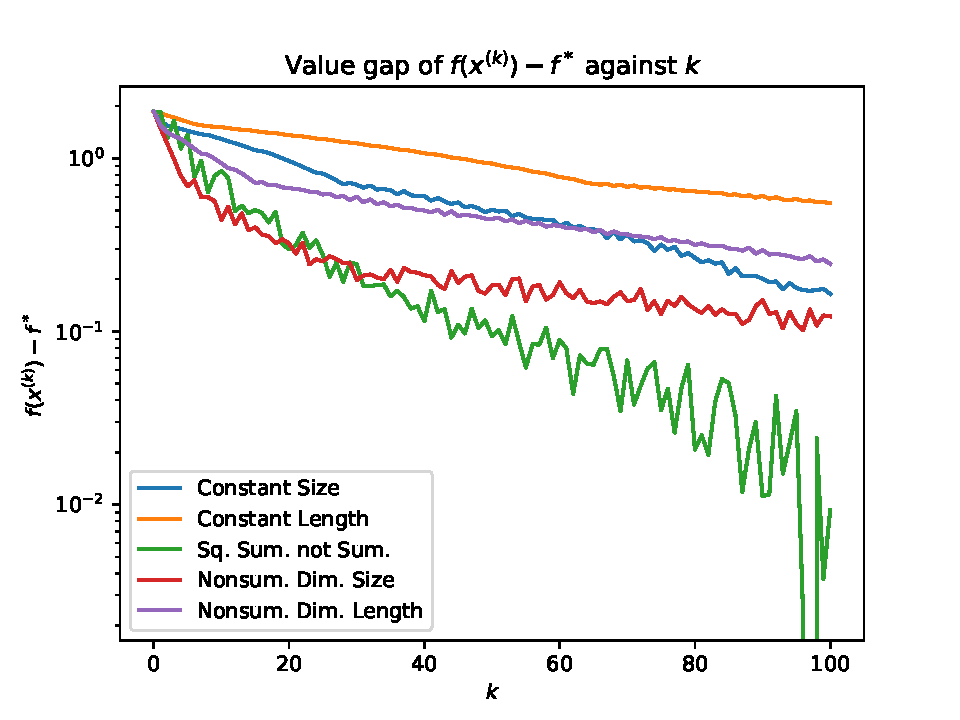
\includegraphics[width = \linewidth]{Figures/Linear Example Value Gap.pdf}
        \caption{Value gap plot}
        \label{fig:linear value gap}
    \end{subfigure}
    \begin{subfigure}{0.49\textwidth}
        \centering
        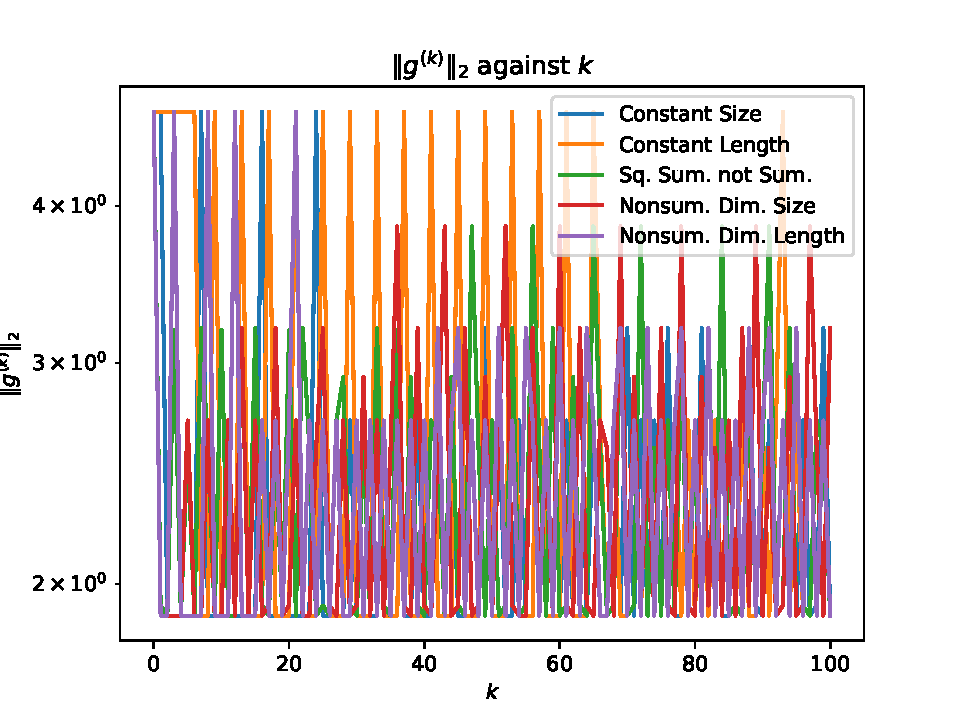
\includegraphics[width = \linewidth]{Figures/Linear Example Subgradient Norm.pdf}
        \caption{Norm subgradient plot}
        \label{fig:linear sg norm}
    \end{subfigure}
    \caption{Plots for the linear problem}
    \label{fig:gd}
\end{figure}
In this case, it happened that the best performing method was using a square summable but not summable approach, however having run it a few times this is not always the case. This may be because of different function geometries behaving in different ways.


\section{LASSO Implementation}\label{sec:lasso}
For the implementation of the life expectancy regression, the data was sourced from \cite{dataset}. In this section we will delve into the code of the LASSO implementation, and in Section \ref{sec:results} we will review the results. The program was implemented in a Jupyter Python notebook.

\subsection{Importing Data and Libraries}
The data was formatted as a CSV file, so Pandas was used in order to import it. The non numerical categories of Country and Status were dropped, since they cannot be used in the linear classifier. There were also a fair number of entries that were empty due to the data being unavailable. As described by \cite{dataset}, this was mostly the case for very small countries. SciKit Learn was used to split the data into a training and testing dataset. While it also includes a LASSO implementation, the point of this entire exercise is to gain familiarity, so LASSO was implemented from scratch.
\begin{minted}{python}
import numpy as np
import pandas as pd
from sklearn.model_selection import train_test_split
import matplotlib.pyplot as plt
import math

data = pd.read_csv("Life Expectancy Data.csv")
data = data.drop(["Country", "Status"], axis=1)
data = data.dropna()

X = data.drop("Life expectancy ", axis = 1)
y = data["Life expectancy "]

X_train, X_test, y_train, y_test = train_test_split(X, y, test_size = 0.25)
\end{minted}

\subsection{LASSO Regression Object}
For convenience, the LASSO Regression and classifier were wrapped together into an object. This object makes working with different LASSO regression using different step sizes much easier. The \verb|train| and \verb|update_weights| methods are pretty simple, as well as the \verb|predict| method implementing a very simple linear classification, as described in Section \ref{sec:define lasso problem}. The method for \verb|subgradient| is a direct adaptation of \eqref{eq:lasso subgradient}, and \verb|lasso_estimate| derived from \eqref{eq:lasso estimate compact}.
\begin{minted}{python}
class LassoRegression():
    def __init__(self, name, p, beta, step_size, l1_penalty):
        self.name = name
        self.p = p
        self.beta = beta
        self.l1_penalty = l1_penalty
        self.step_size = step_size
    
    def train(self, X_train, y_train, maxiter):
        self.X_means = X_train.mean()
        self.X_std = X_train.std()
        self.y_mean = y_train.mean()
        self.y_std = y_train.std()

        estvec = []
        gvec = []
        bestbeta = self.beta
        minest = math.inf
        for k in range(1, maxiter+1):
            est, g = self.update_weights(X_train, y_train, k)
            estvec.append(est)
            gvec.append(np.linalg.norm(g))
            if estvec[-1] < minest:
                minest = estvec[-1]
                bestbeta = self.beta
            if k % 25 == 0:
                print(f"Finished {k} out of {maxiter} iterations on {self.name}")
        self.beta = bestbeta
        return estvec, gvec

    def update_weights(self, X, y, k):
        est = self.lasso_estimate(X, y)
        g = self.subgradient(X, y)
        self.beta -= self.step_size(g, k) * g
        return est

    def predict(self, X):
        norm_X = (X.sub(self.X_means, axis = 1)).div(self.X_std, axis = 1)
        norm_y = norm_X.dot(self.beta)
        return (norm_y * self.y_std) + self.y_mean
    
    def subgradient(self, X, y):
        norm_X = (X.sub(self.X_means, axis = 1)).div(self.X_std, axis = 1)
        norm_y = (y - self.y_mean) / self.y_std
        n = len(norm_y)
        sum = np.sum(norm_X, axis=0)
        g = np.multiply(np.linalg.norm(norm_y-norm_X.dot(self.beta)),sum)*2/n
        g += np.sign(self.beta)*self.l1_penalty
        return g
    
    def lasso_estimate(self, X, y):
        norm_X = (X.sub(self.X_means, axis = 1)).div(self.X_std, axis = 1)
        norm_y = (y - self.y_mean) / self.y_std
        pred = norm_X.dot(self.beta)
        return np.linalg.norm(norm_y-pred)**2
\end{minted}

\subsection{Step Sizes}
This section was duplicated from Section \ref{sec:linear example step sizes} verbatim, with only some tuning as to the constants chosen.
\begin{minted}{python}
def constant_step_size(g, k):
    alpha = 1
    return alpha

def constant_step_len(g, k):
    gamma = 1
    norm = np.linalg.vector_norm(g)
    return gamma/norm

def square_sum_not_sum(g, k):
    a = 10
    b = 1
    return a/(b+k)

def nonsum_dim_size(g, k):
    a = 2
    return a / math.sqrt(k)

def nonsum_dim_len(g,k):
    a = 2
    gammak = a / math.sqrt(k)
    norm = np.linalg.vector_norm(g)
    return gammak/norm
\end{minted}

\subsection{Training and Testing the Model}
Here the code was very simple, only needing to instatiate the \verb|LassoRegression| object and call the methods on it. While experimenting with different step size constants and \(\lambda\) values the print statement was included to monitor the performance of the classifier on the final data set using the LASSO estiamte.
\begin{minted}{python}
p = len(X_train.columns)
beta = np.random.standard_normal(p)
models = [
    LassoRegression("Constant Size", p, beta.copy(), constant_step_size, 1e-1),
    LassoRegression("Constant Length", p, beta.copy(), constant_step_len, 1e-1),
    LassoRegression("Sq. Sum. not Sum.",p,beta.copy(),square_sum_not_sum,1e-1),
    LassoRegression("Nonsum. Dim. Size", p,beta.copy(),nonsum_dim_size,1e-1),
    LassoRegression("Nonsum. Dim. Length",p,beta.copy(),nonsum_dim_len,1e-1)]
maxiter = 50

train_results = [model.train(X_train, y_train, maxiter) for model in models]
test_lassos = [model.lasso_estimate(X_test, y_test) for model in models]
print(test_lassos)
\end{minted}

\subsection{Graphing}
The final section of code simply generates a graph displaying the LASSO estimate with each iteration, as well as one that displays the norm of the gradients on each iteration. The result is Fig. \ref{fig:lasso results}.
\begin{minted}{python}
karr = list(range(1, maxiter + 1))

fig, ax = plt.subplots()
for i in range(len(models)):
    ax.plot(karr, train_results[i][0], label=models[i].name)
ax.set_title("LASSO estimates against $k$")
ax.set_ylabel("LASSO estimates")
ax.set_xlabel("$k$")
ax.set_yscale('log')
ax.legend()

fig2, ax2 = plt.subplots()
for i in range(len(models)):
    ax2.plot(karr, train_results[i][1], label=models[i].name)
ax2.set_title("Norm subgradients against $k$")
ax2.set_ylabel("$\\|g\\|_2$")
ax2.set_xlabel("$k$")
ax2.legend()

plt.show()
\end{minted}


\section{Numerical Results}\label{sec:results}
\begin{figure}[htbp]
    \centering
    \begin{subfigure}{0.49\textwidth}
        \centering
        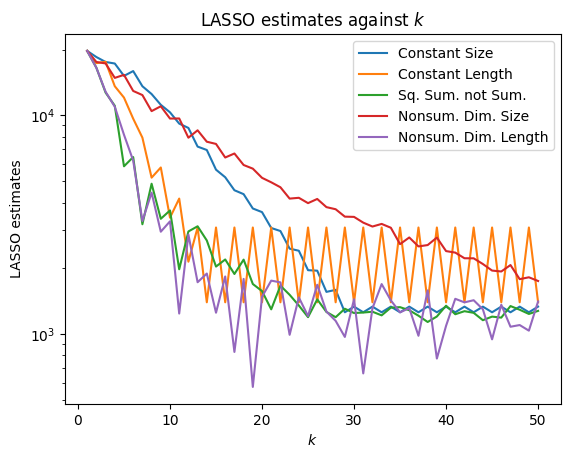
\includegraphics[width = \linewidth]{Figures/LASSO output.png}
        \caption{LASSO estimate during optimization}
        \label{fig:lasso estimates}
    \end{subfigure}
    \begin{subfigure}{0.49\textwidth}
        \centering
        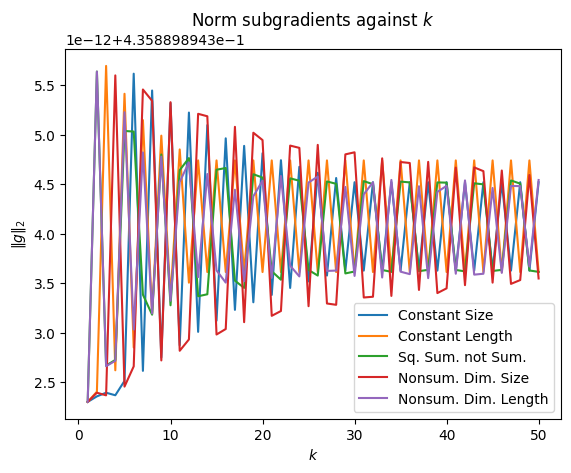
\includegraphics[width = \linewidth]{Figures/LASSO norm grads.png}
        \caption{LASSO norm subgradient plot}
        \label{fig:lasso sg norm}
    \end{subfigure}
    \caption{Plots for the LASSO regression}
    \label{fig:lasso results}
\end{figure}
We can examine our results a little more closely. We can note that just like our results in Section \ref{sec:linear example figs}, the most recent value is not always the best value, because we are using subgradient methods, which are not descent methods. We can also see oscillitory behavior at the end of the curves. This is presumably oscillating because one or more of the values of \(\hat{\beta}_j\) are bouncing around zero on every iteration. Regardless, this is why we made sure during training to save the best \(\hat{\beta}\), to ensure the best possible performance. We can also compare the convergence behaviors of our different methods. We see that nonsummable diminishing size converges the most slowly, followed by constant step size. The other methods converge at roughly the same speed, but nonsummable diminishing step length manages to find the best solution out of all the methods. Constant length seems to plateau with large oscillations at a worse solution than the other methods in this case, but this was not the case everytime that the program was run. Some of these methods might be able to have better performance depending on the starting point randomly chosen and with finer tuning of the constants, but with limited time for this project these were the values we settled on.

\section{Conclusion}\label{sec:conclusion}
Subgradients and subgradient methods are a very versatile way of optimizing a wide variety of problems where traditional gradient-based methods cannot be used. A great example of an application is a LASSO regression scheme, which employs the non-differentiable \(L_1\) norm. As demonstrated in this project, using these two together is an effective way to build a linear classifier for a given dataset. This project proved difficult at times, and certainly provided a challenge, but was ultimately very informative and educational.

\appendix
\subsection{Source Code Availablility}\label{sec:github}
The source code for this project, including the code for this \LaTeX{ }document, is available on GitHub: \url{https://github.com/Derpanieux/Convex-Optimization-Term-Project}. 

\subsection{Proving Subgradient Properties}\label{sec:subgradient properties proofs}
\subsubsection{When the Function is Differentiable}
We can begin by supposing that \(f\) is differentiable at \(x\), and therefore \(\nabla f(x)\) exists. Let us write a definition for each of its elements
\begin{equation}\label{eq:gradient elementwise def}
    \nabla f_i(x) = \lim_{y \rightarrow x} \frac{f(y)-f(x)}{y_i-x_i}
\end{equation}
And let us also rewrite \eqref{eq:modified subgradient def} with an elementwise sum
\begin{equation}\label{eq:subgradient elementwise sum}
f(x) - f(y)+ \sum^{n}_{i=1} g^T_i(y_i-x_i) \leq 0
\end{equation}
We can combine \eqref{eq:gradient elementwise def} and \eqref{eq:subgradient elementwise sum}
\begin{equation}
\lim_{y \rightarrow x} f(x) - f(y)+ \sum^{n}_{i=1} \nabla f_i(x)^T(y_i-x_i) \leq 0
\end{equation}
Substitute and simplify and we find that
\begin{equation}
\lim_{y \rightarrow x} f(x) - f(y)+ \sum^{n}_{i=1} \nabla f_i(x)^T(y_i-x_i) = 0
\end{equation}
If we are interested in trying an alternate \(g \neq \nabla f_i(x)\), we can say that a particular \(g_i\) would be invalid if
\begin{equation}\label{eq:differentiable cookie}
g_i(y_i-x_i) > \nabla f_i(x)(y_i-x_i)
\end{equation}
If \(g_i > \nabla f_i(x)\) and \(y_i > x_i\), this condition is fulfilled and therefore no values of \(g_i > \nabla f_i(x)\) are valid. Likewise, if \(g_i < \nabla f_i(x)\) and \(y_i < x_i\) this condition is fulfilled and therefore no values of \(g_i < \nabla f_i(x)\) are valid. Therefore the only valid values for every \(g_i = \nabla f_i(x)\), so the only valid \(g = \nabla f(x)\) if \(\nabla f(x)\) exists.

\subsubsection{Global Minimum}
If \(x^*\) is a global minimum it must be true that \(\forall y \in \dom f\)
\begin{equation}\label{eq:global min def}
f(x^*) \leq f(y)
\end{equation}
If we have \(g\) equal to the zero vector in \eqref{eq:subgradient def}, we end up removing the second term, so we end up with
\begin{equation}\label{eq:zero vector subgradient}
f(y) \geq f(x)
\end{equation}
We can trivially redefine \(x = x^*\) to derive \eqref{eq:global min def}. Therefore \(x^*\) is optimal if and only if the zero vecctor is included in its subdifferential.

\subsubsection{Convexity}
We can view \eqref{eq:modified subgradient def} as defining a halfspace in terms of \(x, y, f\). From \eqref{eq:math subdifferential} we can see that \(\partial f(x)\) is composed of intersections of these halfspaces. Since halfspaces are always convex and the intersection of convex sets is always convex, \(\partial f(x)\) must be a convex set.

\bibliographystyle{IEEEtran}
\bibliography{refs}

\end{document}